A study of the role of the fiber diameter in tritium detection was carried out. Simulations of a single $20~\cm$ length scintillating fiber and two different diameters, $1~\mm$ and $2~\mm$ (the commercial options given for Saint-Gobain), were compared. An important point is the relation between fiber diameter and the cosmic ray detection. The energy deposited a the scintillating fiber by cosmic rays is proportional to the active volume so, the cosmic ray signal would be larger for $2~\mm$ diameter fibers. The objective of this study is to find the background in the energy up to $18~\keV$. The tritiated water source was replaced by a cosmic ray source generated by the CRY library\footnote{CRY library, Cosmic-Ray Shower library} \cite{CRYwebsite, CRYpaper} is a package implemented in C++. This library generates cosmic-ray showers for different particles (muons, neutrons, protons, electrons, photons and pions). The cosmic source employed is a horizontal square of $1 \times 1~\meter ^2$ located $35~\cm$ over the detector with the typical distribution of cosmic particles at sea level. The distributions of energy deposited in the scintillating fibers for $1~\mm$ and $2~\mm$ diameters by cosmic rays are shown in Figure \ref{fig:DiameterComparison}. As can be seen in the figure, a background about $50\%$ smaller is obtained for $1~\mm$ fiber diameters, which implies a smaller detector MDA. There are other reasons that may favor $2~\mm$ fibers, such as their greater rigidity and better flow of water through them. Thus, a complementary experimental study is needed to assess the most appropriate scintillating fibers diameter.

\begin{figure}[hbtp]
\centering
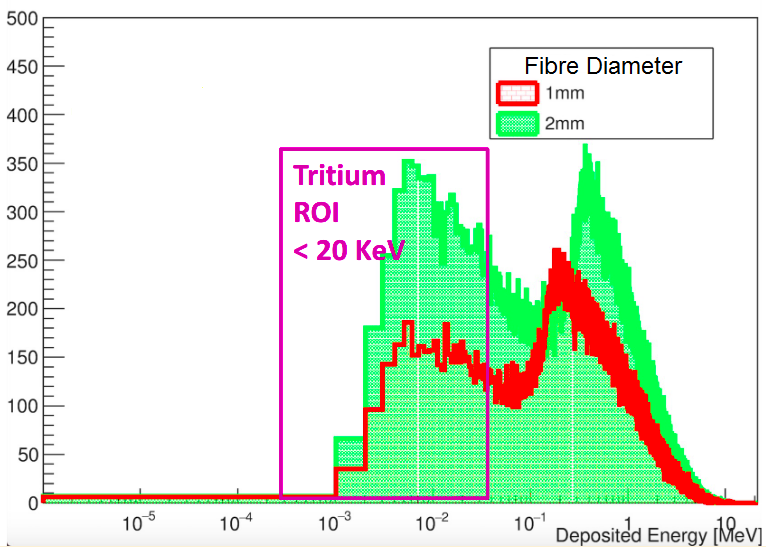
\includegraphics[scale=0.4]{6Simulations/61TRITIUMDesign/614Diameter/ComparisonDiameter.png}
\caption{Comparison of the energy deposition by cosmic rays in scintillating fibers of $1~\mm$ and $2~\mm$ diameter.\label{fig:DiameterComparison}}
\end{figure}o